\documentclass[conference]{IEEEtran}
\IEEEoverridecommandlockouts

\usepackage{cite}
\usepackage{amsmath,amssymb,amsfonts}
\usepackage{graphicx}
\usepackage{float}
\usepackage{textcomp}
\usepackage{xcolor}
\usepackage{url}

\begin{document}

\title{A Deep Learning Approach for Smartphone Screen Glass Defect Detection Using CNN}

\author{
\IEEEauthorblockN{Abubakar Siddiq Sazzad}
\IEEEauthorblockA{
Department of Computer Science and Engineering \\
International University of Scholars \\
Email: siddiqsazzad001@gmail.com
}
}

\maketitle

\begin{abstract}
Quality inspection is a critical stage in modern smartphone manufacturing. Detecting defects in screen glass components is essential to maintain product reliability and customer satisfaction. Traditional manual inspection is time-consuming, inconsistent, and prone to human error. This research presents a deep learning-based image classification system for detecting smartphone screen glass defects using Convolutional Neural Networks (CNNs). The model was trained using the Smartphone Screen Glass Dataset (SSGD), which contains 2,504 images representing defective and non-defective screen glass samples. A transfer learning approach based on MobileNetV2 was implemented using the TensorFlow framework and trained on Google Colab GPU resources. Images were resized to 224×224 pixels and augmented to improve model generalization. Experimental results demonstrate that CNN-based models can effectively identify defects with an accuracy of approximately 90.9\%, highlighting the potential of deep learning methods for automated industrial inspection systems.
\end{abstract}

\begin{IEEEkeywords}
Deep Learning, Convolutional Neural Networks, Image Classification, Defect Detection, MobileNetV2, Industrial Inspection
\end{IEEEkeywords}

\section{Introduction}

Quality control plays an essential role in modern manufacturing industries. In smartphone production, screen glass components are particularly vulnerable to defects such as scratches, cracks, and surface contamination. These defects may occur during manufacturing, packaging, or transportation. Even small imperfections can affect the usability and reliability of the final product.

Traditionally, visual inspection of smartphone screens is performed manually by trained operators. However, manual inspection suffers from several limitations including fatigue, inconsistent decision-making, and difficulty detecting subtle defects. As production scales increase, the need for automated inspection systems becomes increasingly important.

Recent advances in artificial intelligence and computer vision have enabled automated visual inspection systems using deep learning techniques. Convolutional Neural Networks (CNNs) have demonstrated exceptional performance in image classification and pattern recognition tasks by automatically learning hierarchical features from raw image data.

This research proposes a CNN-based deep learning approach to detect smartphone screen glass defects using the SSGD dataset.

\section{Motivation}

The growing demand for high-quality smartphones requires efficient inspection methods capable of detecting defects quickly and accurately. Manual inspection introduces several challenges:

\begin{itemize}
\item High labor cost
\item Human fatigue and inconsistent inspection results
\item Difficulty detecting small defects
\item Limited scalability in mass production
\end{itemize}

Deep learning provides a promising solution by enabling automated defect detection systems capable of analyzing images rapidly and consistently.

\section{Problem Statement}

Detecting smartphone screen defects using computer vision presents several challenges:

\begin{itemize}
\item Surface reflections and lighting variations
\item Small or subtle defect patterns
\item Limited labeled datasets
\item Class imbalance between defective and non-defective samples
\end{itemize}

The goal of this research is to develop a CNN-based classification model capable of accurately identifying smartphone screen glass defects.

\section{Objectives}

The primary objectives of this research include:

\begin{itemize}
\item Develop a deep learning model for defect detection
\item Train a CNN-based image classification system
\item Apply transfer learning using MobileNetV2
\item Evaluate performance using classification metrics
\end{itemize}

\section{Related Work}

Deep learning has significantly improved computer vision applications including object detection and image classification. CNN architectures such as AlexNet, VGGNet, ResNet, and MobileNet have achieved state-of-the-art results on large-scale image datasets.

Transfer learning allows pre-trained networks to be adapted to domain-specific tasks with limited data. In industrial inspection systems, CNN-based models have been successfully used to detect defects in metal surfaces, fabrics, and electronic components.

\section{Dataset and Preprocessing}

The dataset used in this research is the Smartphone Screen Glass Dataset (SSGD), which contains 2,504 images.

The dataset includes both defective and non-defective smartphone screen glass samples captured under controlled conditions.

Images were resized to 224×224 pixels and normalized before training.

\subsection{Data Augmentation}

To improve model generalization and prevent overfitting, several data augmentation techniques were applied:

\begin{itemize}
\item Random rotation
\item Random brightness adjustment
\item Image normalization
\end{itemize}

\section{Methodology}

The proposed defect detection system is based on a Convolutional Neural Network with transfer learning.

MobileNetV2 was used as the base model for feature extraction. The architecture consists of:

\begin{itemize}
\item Pre-trained MobileNetV2 layers
\item Global average pooling layer
\item Fully connected dense layer
\item Softmax classification layer
\end{itemize}

Transfer learning allows the model to leverage previously learned visual features from the ImageNet dataset.

\section{Experimental Setup}

The system was implemented using TensorFlow and trained on Google Colab GPU.

\begin{table}[H]
\centering
\begin{tabular}{|c|c|}
\hline
Parameter & Value \\
\hline
Image Size & 224×224 \\
Batch Size & 32 \\
Optimizer & Adam \\
Epochs & 10 \\
Framework & TensorFlow \\
Hardware & Google Colab GPU \\
\hline
\end{tabular}
\caption{Model Training Configuration}
\end{table}

\section{Training Performance}

The model was trained for multiple epochs using the Adam optimizer. Figure~\ref{fig:training} shows the training process.

\begin{figure}[H]
\centering
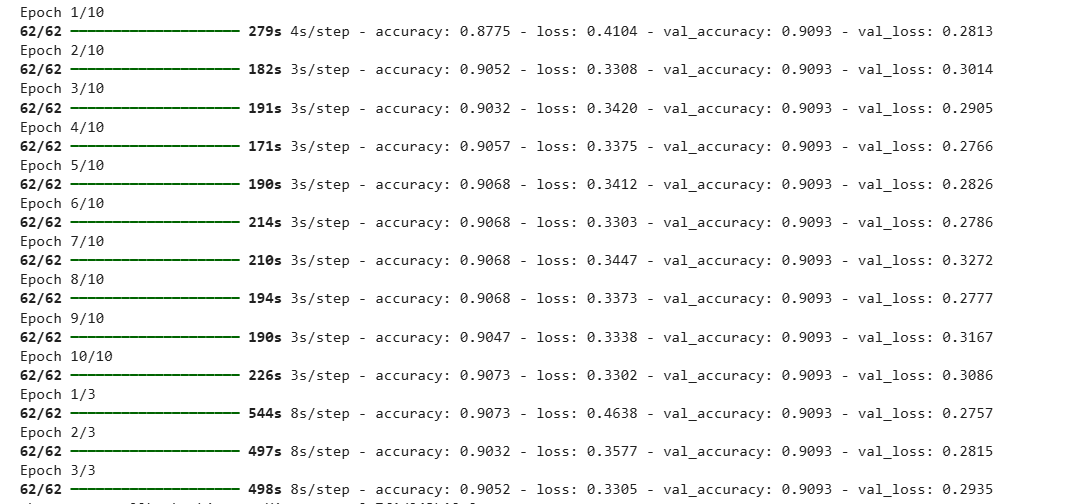
\includegraphics[width=0.45\textwidth]{training_epochs.png}
\caption{Training and Validation Accuracy}
\label{fig:training}
\end{figure}

\section{Confusion Matrix Analysis}

The confusion matrix provides a visual representation of classification performance.

\begin{figure}[H]
\centering
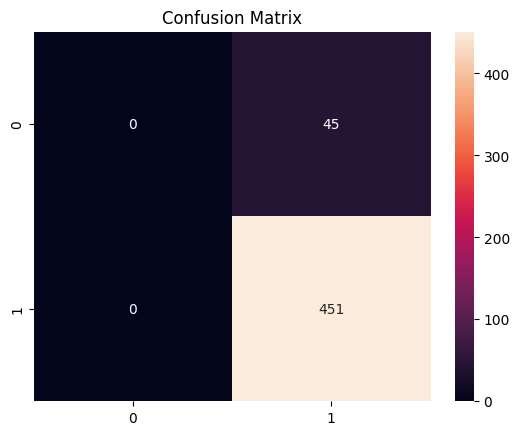
\includegraphics[width=0.45\textwidth]{confusion_matrix.png}
\caption{Confusion Matrix}
\label{fig:confusion}
\end{figure}

\section{Performance Evaluation}

The model achieved the following performance metrics on the validation dataset.

\begin{table}[H]
\centering
\begin{tabular}{|c|c|}
\hline
Metric & Value \\
\hline
Accuracy & 90.93\% \\
Precision & 0.91 \\
Recall & 1.00 \\
F1 Score & 0.95 \\
\hline
\end{tabular}
\caption{Model Performance Metrics}
\end{table}

\section{Discussion}

Although the model achieved high overall accuracy, the confusion matrix indicates class imbalance within the dataset. The model tends to predict the majority class more frequently. Future improvements may involve dataset balancing techniques such as oversampling or class weighting.

\section{Future Work}

Future research may explore:

\begin{itemize}
\item Larger datasets
\item Object detection frameworks such as YOLO
\item Lightweight models for edge deployment
\item Explainable AI techniques
\end{itemize}

\section{Conclusion}

This research presented a CNN-based deep learning approach for smartphone screen glass defect detection using the SSGD dataset. The MobileNetV2-based model achieved strong classification performance with approximately 90.9\% accuracy. The results demonstrate the potential of deep learning techniques for automated industrial inspection systems.

\begin{thebibliography}{00}

\bibitem{b1} M. Tan and Q. Le, “EfficientNet: Rethinking Model Scaling for CNNs,” ICML, 2019.

\bibitem{b2} A. Howard et al., “MobileNets: Efficient CNNs for Mobile Vision Applications,” 2017.

\bibitem{b3} K. Simonyan and A. Zisserman, “Very Deep Convolutional Networks,” ICLR, 2015.

\bibitem{b4} K. He et al., “Deep Residual Learning for Image Recognition,” CVPR, 2016.

\bibitem{b5} A. Krizhevsky et al., “ImageNet Classification with Deep CNNs,” NIPS, 2012.

\bibitem{b6} J. Deng et al., “ImageNet: A Large-Scale Hierarchical Image Database,” CVPR, 2009.

\bibitem{b7} F. Chollet, “Xception: Deep Learning with Depthwise Separable Convolutions,” CVPR, 2017.

\bibitem{b8} D. P. Kingma and J. Ba, “Adam: A Method for Stochastic Optimization,” ICLR, 2015.

\bibitem{b9} TensorFlow Documentation, https://www.tensorflow.org

\bibitem{b10} Keras Documentation, https://keras.io

\end{thebibliography}

\end{document}